%\documentclass[a4paper]{article}
\documentclass{article}
%\documentclass[journal]{IEEEtran}
%\documentclass{report}
%\documentclass{ActaOulu}

\usepackage{graphicx}
\usepackage{multirow}
\usepackage{authblk}
\usepackage{float}
\usepackage{rotating}
\usepackage{url}
\usepackage{lscape}
\usepackage{longtable}
\usepackage{subfig}
\usepackage{natbib}
\usepackage{lineno}
\usepackage{amsmath}
\usepackage{epsfig}
\usepackage{caption}
\usepackage{latexsym}
\usepackage[a4paper]{geometry}
%\setlength{\captionmargin}{20pt}
%\usepackage{graphicx}
%\usepackage[all,knot]{xy}
%\xyoption{arc}
%\usepackage{url}
%\usepackage{multimedia}
%\usepackage{hyperref}
\linespread{1.6}
%\linespread{1.2}

\newcommand{\Deg}{$^{\circ}$}
\newcommand{\Pic}[2][0.85]{\begin{center}\includegraphics[width=0.8\textwidth,height=#1\textheight,keepaspectratio]{#2}
 \end{center} }
%\newcommand{\captionfonts}{\small}
%%%%%%%%%%%%%%%%%%%%%%%%%%
% Different font in captions
\newcommand{\captionfonts}{\small}

\makeatletter  % Allow the use of @ in command names
\long\def\@makecaption#1#2{%
 \vskip\abovecaptionskip
 \sbox\@tempboxa{{\captionfonts #1: #2}}%
 \ifdim \wd\@tempboxa >\hsize
   {\captionfonts #1: #2\par}
 \else
   \hbox to\hsize{\hfil\box\@tempboxa\hfil}%
 \fi
 \vskip\belowcaptionskip}
\makeatother   % Cancel the effect of \makeatletter
%%%%%%%%%%%%%%%%%%%%%%%%%%%%
\begin{document}
\section{Stochastic numeric methods}
To account for the impact of the uncertainty in the parameters, it is natural to consider moments
of the solutions over the probabilistic space. In other words, we need to evaluate multi-dimensional
integrals (Gaobrowndiffeqn). The main idea of the stochastic collocation approach is to abandon the 
random sampling approach and consider the use of the more advanced integration approaches as 
hierarchical integration techniques.

We are interested in convergence of the first and second moment of the model output when using sparse
grid as a colocation method. In an attempt to minimize the number of sample points we use sparse grid
schemes. The colocation points in the high-dimensional random parameters space is significantly reduced 
compared to a full tensor product. 

The MC, LHS, PCQ and SP approaches follow identical procedures except in the 
choice of grid points in the sample space and the quadrature weights associated with those 
points. These procedures and the choices of collocation points for the SP are described below.

\subsection{Monte Carlo simulations}
In a typical MC simulation with $N_{MC}$ number of samples the mean converges asymptotically as 
$\sqrt{N_{MC}^{-1}}$, and is independent of the number of random dimensions, $N$ (linpacificlab).
The general procedure for MC simulation of transport equations is:
\begin{itemize}
\item Generate $N_{MC}$ sample
\item Solve the deterministic problem for each sample
\item Stochastic moments are computed as simple arithmetic means
\begin{equation}
\langle U(\xi_{i=1\cdots N_{MC}})^N\rangle = \frac{1}{N_{MC}}\sum_{i=1}^{N_{MC}}U(\xi_i)^N
\end{equation}
The mean is given as mean(U) = $\langle$ U $\rangle$. By the central limit theorem (Chung, and more)
the accuracy is $\frac{\sigma}{\sqrt{N_{MC}}}$, where $\sigma$ is the standard deviation of the estimate. 
Thus to double the accuracy, it is necessary to quadruple the number of sample points (keithpaper). 
\end{itemize}

\subsection{Latin Hypercube Sampling}
The Latin Hypercube Sampling is implemented as bellow:
\begin{itemize}
\item For each random dimension/variable generate $N_{pts}$, using a method improved by (keithpaper)
\item For every $i=1,\cdots,N_{pts}$ points, one value from each of the $N_{dir}$ random direction is taken
to form the coordinates of the point in the $N_{dir}$-dimensional sample space.
\item Evaluate the model for this value of the sample space.
\item Expectations and other statistics are calculated as in MC. 
\end{itemize}

\subsection{PCQ}
PCQ is natural evolution of the SG, only that the evaluation of the projections is performed 
through quadrature - that is, via numerical rather than analytical integration. 
It leads to a method that has the simplicity of MC and cost of PC. A detailed explanation
can be found in (keithspaper).

\subsection{Sparse grid collocation method}
%Means, variances, and higher moments of random variables are integrals. These integrals must be
%computed numerically for large-scale systems, and thus, because of the ``curse of dimensionality",
%become problems of efficiently sampling a multi-dimensional random space (mitsppdf). Numerical
%integration is a problem of efficiently characterizing a function over a space by sampling it at discrete
%points: $\int f(x) dx \approx \sum_i w_if(x_i)$. 
\subsubsection{One dimension}
%To find an approximate solution, one possible approach is Monte Carlo simulation. Other strategies
%like Riemann sums with regularly-spaced modes are also straightforward.
A general univariate integration problem can be written as :
\begin{equation}
I[g] = \int_{\Omega} g(x) w(x) dx
\end{equation}
Where $x$ represents a random variable, $g(x)$ is a function in $x$ and $w(x)$ 
represents the p.d.f. of $x$ with support $\Omega$.
The polynomial-based approaches fit polynomials to the integrand, and the resulting polynomial 
function is then integrated. In general, the nodes are the roots of the fitted polynomials.
A sequence of quadrature rule is defined $V = \{V_i : i\in N\}$ and each
 rule $V_i$ specifies a set of rule $X_i \subset R$ and a corresponding weight 
 function $w_i :X_i \longrightarrow R$ . The optimal abscissas of the
 $n-$point Gaussian quadrature formulas are the roots of an orthogonal polynomial
 for the same interval and weighting function. In this case the approximation of $I$ by $V_i$ 
 is given as : 
\begin{equation}
V_i[g] =\sum_{x \in X_i}g(x) w_i(x) dx
\end{equation}

\textbf{Gauss-Legendre } \\ 
Gaussian quadrature is the best known polynomial-based method, famed for its $2n-1$ degree of 
polynomial exactness, meaning that with $n$ function evaluations, all integrands which are 
polynomials of order $2n -1$ or less will be integrated exactly. Gaussian quadrature utilizes 
orthogonal polynomials, such as Legendre, Hermite, or Laguerre polynomials. When approximating
expectations of functions of random variable, the choice of orthogonal polynomial should reflect the
type of random variable. Legendre polynomials should be used for uniform random variables, and 
Hermite polynomials for normal random variables. However, the Gauss-Legendre formulas are in
general not nested.\\

\textbf{Gauss-Kronrod-Patterson quadrature rules}\\
Gauss-Kronrod-Patterson (citation) quadrature are an extension of Gaussian rules first developed by
Kronrod and then iterated by Patterson to yield a sequence of nested quadratures: the set of
nodes for each level are contained in the nodes for all successive levels. In the sparse grid 
formulation nesting allows function evaluations to be reused. 
Thus, the $n$-point Gauss quadrature formula was extended by $n+1$ points (zeros of the Stieltjes
polynomials such that the polynomials) degree of exactness or the resulting $2n+1$ formula is maximal.\\

\textbf{Clenshaw-Curtis}\\
The nodes of Clenshaw-Curtis (citation) quadrature are at the roots of Chebyshev polynomials and
is exact for polynomial of order n when $n+1$ points are used.
For a given level $k \in N$ the sequence of $n_l$-point quadrature formula is:
\begin{equation}
n_k= \left \{ \begin{array}{ll}
                    2^{k-1} + 1 & \mbox{if $k>1$}\\
                    1 &\mbox{if $k=1$}
              \end{array}
              \right.
\end{equation}
And the abscissas are given by:
\begin{equation}
x_{ki}= \left \{ \begin{array}{ll}
                   -\frac{1}{2}\cdot(\cos\frac{\pi \cdot (i-1)}{n_k-1}+1) & \mbox{for $k=1,\cdots,n_k$, if $n_k >1$}\\
                    1 &\mbox{for $k=1$, if $n_k=1$}
              \end{array}
              \right.
\end{equation}

When considering the efficiency of the integration measured through polynomial exactness, it is
worth keeping in mind that polynomial exactness is just one measure of accuracy and making
other choices may well better highlight the advantages of other methods. It was shown by (Threfethen 
and Gaobrown) that the Clenshaw-Curtis very often is comparable or even better in accuracy to Gauss
quadrature despite formally having lower polynomial exactness. This behavior will be observed 
in section 4 in the construction of the hazard map.

\subsubsection{Multiple dimensions}
The extension of the univariate quadrature rules to multiple dimensions can be achieved by 
the product rule. 

\textbf{Full Grids}\\
 The use of a full tensor product space is attractive in the case of a small number of random variables.
 In D dimensions, the number of evaluations of the function grows exponentially and as dimension
 grows, the error order grows as well at an exponential rate: $\mathcal{O}(n_{q}^{-r/D})$.
 This is defined for functions in $C^r$ (function with bounded mixed derivatives up to order r)
 and where $n_q$ is the total number if points in the grid.
 If the number of random variables is moderate or large, one should rather consider full polynomial 
 space or sparse tensor product spaces. 

 \textbf{Sparse Grids}\\
 Smolyak (1963) introduced what is now known as Smolyak's formula and is the underlying formulation
 of all sparse grid methods (MITsp and more). Define the level $i$ difference quadrature:
 \begin{equation}
\Delta_i = V_i - V_{i-1},  \; V_0 = 0 \; \forall i \in N
\end{equation}
With $\textbf{i} = [i_1, \cdots, i_D]$, define for any $q \in N_0$:
 \begin{equation}
N_q^D = \lbrace \textbf{i} \in N^D : \sum_{d=1}^{D} i_d=D + q \rbrace 
\end{equation}
and $N_{q}^D = \emptyset$ for $q \le 0$. \\
 The Smolyak rule with accuracy level $k \in N$ for D-dimensions:
 \begin{equation}
A_{D,k}[g] = \sum_{q=0}^{k-1}\sum_{\textbf{i}\in N_{q}^D} (\Delta_{i_1} \otimes \cdots \otimes \Delta_{i_D})[g]
\end{equation}
The above rule was improved by (Wasilowki) by expressing $A_{D,k}[g]$ directly
in terms of the univariate quadrature rules instead of their differences.
\begin{equation}
A_{D,k}[g] = \sum_{q=k-D}^{k-1}(-1)^{k-1-q}\begin{pmatrix}D-1 \\ k-1-q \end{pmatrix}
\sum_{i \in N_q^D}(V_{i_1} \otimes \cdots \otimes V_{i_D})[g]
\end{equation}
 It can be seen that nesting causes points of different grids in the sum to coincide, and the number of
 common points increases with both the level and dimension of the sparse grid (Fig.~\ref{fig1}).
 The error for a sparse grid can be estimate in the same fashion as the full grid case:
 \begin{equation}
\lvert I[g] -A_{D,q}[g] \rvert = \mathcal{O}(n_{q}^{-r}\log(n_q)^{(D-1)(r+1)})
\end{equation}
 The advantage of the stochastic collocation approach on sparse grids with respect to, e.g., Monte Carlo 
 simulation, is to reduce the number of solver calls.
 The Smolyak algorithm provides a way to construct interpolation functions based on a minimal number
 of points in multi-dimensional space. When one is dealing with multiple stochastic dimensions, it is 
 straightforward to extend the interpolation functions in the one dimension to multiple dimensions by 
 using tensor products in this special way (hierarchicalxiangma, klimkethesis, Melosh07). The algorithm 
 provides a linear combination of tensor products chosen in such a way that the interpolation error is 
 nearly the same as the full-tensor product in higher dimensions. 
 %As the dimension of the problem increases the number of points required can be several order of
 %magnitude different. \\
\begin{figure}[H]
      \begin{minipage}[b]{0.6\textwidth}
        \begin{tabular}{c}
       % \Pic[0.3]{SRTM30_dem.jpg}\\
       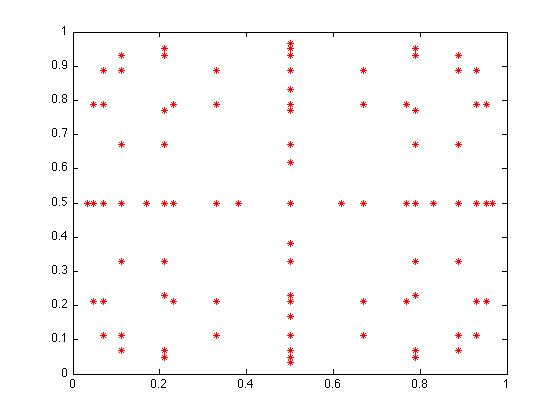
\includegraphics[width=7cm,height=8cm,keepaspectratio]{fig/GQU_2_6.jpg}\\
        (a)
        \end{tabular}
    \end{minipage}
%\hfill
    \begin{minipage}{0.6\textwidth}
        \begin{tabular}{c}
       % \Pic[0.3]{NED30_dem.jpg}\\
	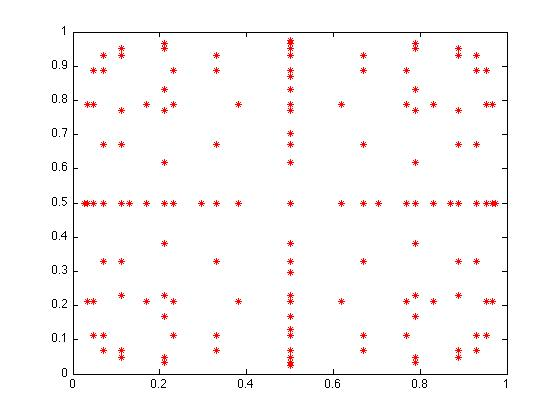
\includegraphics[width=7cm,height=8cm,keepaspectratio]{fig/GQU_2_7.jpg}\\
        (b)
        \end{tabular}
    \end{minipage} 
    \begin{minipage}[b]{0.6\textwidth}
        \begin{tabular}{c}
       % \Pic[0.3]{SRTM30_dem.jpg}\\
       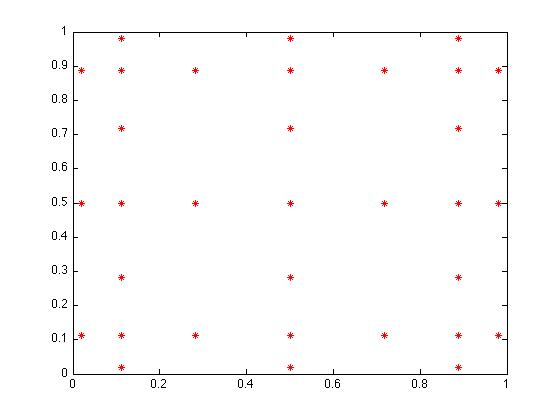
\includegraphics[width=7cm,height=8cm,keepaspectratio]{fig/KPU_2_6.jpg}\\
        (c)
        \end{tabular}
    \end{minipage}
%\hfill
    \begin{minipage}{0.6\textwidth}
        \begin{tabular}{c}
       % \Pic[0.3]{NED30_dem.jpg}\\
	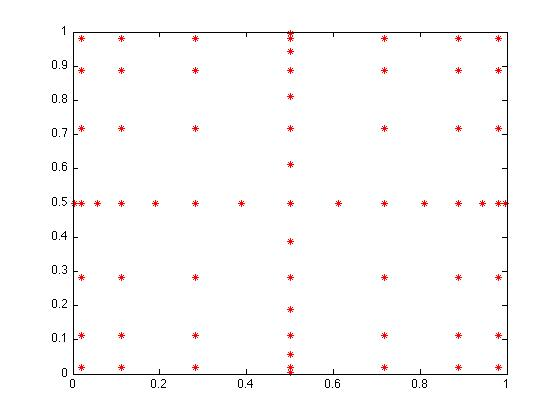
\includegraphics[width=7cm,height=8cm,keepaspectratio]{fig/KPU_2_7.jpg}\\
        (d)
        \end{tabular}
    \end{minipage} 
\caption{(a) Gauss-Legendre level 6 of accuracy
(b) Gauss-Legendre level 7 of accuracy
(c) Kronrod-Paterson level 6 of accuracy
(d) Kronrod-Paterson level 7 of accuracy }
\label{fig1}  
\end{figure}


\end{document}

